% !TeX document-id = {5c05c331-134f-48f1-8db3-fd32c67a647b}
%%%%%%%%%%%%%%%%%%%%%%%%%%%%%%%%%%%%%%%%%
% Journal Article
% LaTeX Template
% Version 2.0 (February 7, 2023)
%
% This template originates from:
% https://www.LaTeXTemplates.com
%
% Author:
% Vel (vel@latextemplates.com)
%
% License:
% CC BY-NC-SA 4.0 (https://creativecommons.org/licenses/by-nc-sa/4.0/)
%
% NOTE: The bibliography needs to be compiled using the biber engine.
%
%%%%%%%%%%%%%%%%%%%%%%%%%%%%%%%%%%%%%%%%%

% Magic comments for TeXStudio
% !TeX program = pdflatex
% !BIB program = biber
% !TeX encoding = utf8
% !TeX spellcheck = en_US

%----------------------------------------------------------------------------------------
%	PACKAGES AND OTHER DOCUMENT CONFIGURATIONS
%----------------------------------------------------------------------------------------

\documentclass[
	a4paper, % Paper size, use either a4paper or letterpaper
	10pt, % Default font size, can also use 11pt or 12pt, although this is not recommended
	unnumberedsections, % Comment to enable section numbering
	twoside, % Two side traditional mode where headers and footers change between odd and even pages, comment this option to make them fixed
]{LTJournalArticle}

% BibLaTeX bibliography file
\bibliography{bibAntoine.bib} 
\bibliography{bibNathan.bib} 
\bibliography{bibSandro.bib}

\runninghead{Real-Time Digital Processing of PPG Signals for Wearable Devices} % A shortened article title to appear in the running head, leave this command empty for no running head

\footertext{} % Text to appear in the footer, leave this command empty for no footer text

\setcounter{page}{1} % The page number of the first page, set this to a higher number if the article is to be part of an issue or larger work

% Main header file
% % % % % % % % % % % % % % % % % % % % % % % % % % % % % % % % % % % % % % % % %
%
% OSTReport -- Additional packages frequently used in reports
%
% % % % % % % % % % % % % % % % % % % % % % % % % % % % % % % % % % % % % % % % %

% Mathematical equations
\usepackage{amsmath}
\usepackage{amssymb}
\usepackage{bm}
\usepackage{MnSymbol}
%\usepackage{breqn}

% Tables
\usepackage{multirow}
\usepackage{tabularx}
\usepackage{booktabs}

% Figures
\usepackage{pdfpages}
\usepackage{epstopdf}
\usepackage{float}
\usepackage{graphicx}
\usepackage{caption}
\usepackage{subcaption}
%\usepackage[outdir=./]{epstopdf}

% Quotation marks
\usepackage{csquotes}
\setquotestyle[quotes]{german}

% Si Units
\usepackage{siunitx}
\sisetup{detect-all,sticky-per,per-mode=symbol}

% Multicolumn documents and sections
\usepackage{multicol}

\PassOptionsToPackage{svgnames,x11names,dvipsnames}{xcolor}
\usepackage[most]{tcolorbox}

%----------------------------------------------------------------------------------------
%	TITLE SECTION
%----------------------------------------------------------------------------------------

\title{Real-Time Digital Processing of PPG Signals for Wearable Devices} % Article title, use manual lines breaks (\\) to beautify the layout

% Authors are listed in a comma-separated list with superscript numbers indicating affiliations
% \thanks{} is used for any text that should be placed in a footnote on the first page, such as the corresponding author's email, journal acceptance dates, a copyright/license notice, keywords, etc
\author{%
	Nathan Hoffman\textsuperscript{1}\thanks{Corresponding author: \href{mailto:nathan.hoffman@students.unibe.ch}{nathan.hoffman@students.unibe.ch} \\ \textbf{Received:} May 2, 2024, \textbf{Published:} \today}, Antoine Biebuyck\textsuperscript{1} \\ 
}

% Affiliations are output in the \date{} command
\date{\footnotesize\textsuperscript{\textbf{1}}ARTORG Center for Biomedical Engineering Research, University of Bern, Bern, Switzerland}

% Full-width abstracta
\renewcommand{\maketitlehookd}{%
	\begin{abstract}
		\noindent In recent times, there has been a desire to monitor vital signs such as heartrate in a continuous and cost-effective manner through use of wearable devices. Photoplethysmography presents itself as a robust technology to accomplish that goal despite its initial drawback of high signal noise. Such noise can be relatively easily removed by the use of well-known digital filtering. Thereafter, a heartbeat detection algorithm can be applied to the filtered signal. While these operations are at first applied to the offline signal, translating the implementation on a microcontroller allows for real-time signal filtering and hearbeat detection. This study presents digital filters that succesfully remove the unwanted noise and an algorithm that successfully counts the peaks of heartbeats. While the filtering was also successfully perfomed in real-time, the heartbeat detection algorithm failed to produce an output when carried out in real-time. Further research will be required to refine the results from this study.
	\end{abstract}
}

%----------------------------------------------------------------------------------------

\begin{document}

\maketitle % Output the title section

%----------------------------------------------------------------------------------------
%	ARTICLE CONTENTS
%----------------------------------------------------------------------------------------

% !TeX encoding = utf8
% !TeX spellcheck = en_US

\section{Introduction}

Lub dub, lub dub, lub dub... Over the course of life, the heart perpetually beats and yet one does not perceive the thump. Nevertheless, the heart beat dictates the rhythm of life. Throughout history, ancient civilizations understood the heart's fundamental force in the preservation of life. Hence, doctors in antiquity had already started to palpate the pulse to extract the rate. \cite{hajar_pulse_2018}

At the present time, palpation of the peripheral arteries still remains a customary clinical technique but several more advanced technologies have also emerged. These include electrocardiography, which measures the electrical activity of the myocardial pathway, magnetic induction tomography, which measures changes of tissue connectivity and impedance, ballistocardiography, which measures the vibrations of the body and phonocardiography, which measures the noise produced by the heart. \cite{ludwig_measurement_2018}

Despite the respective abilities of the above instrumentation to accurately measure heart rate, they possess several disadvantages, particularly concerning their integration into wearable devices. For example, electrocardiography has a complicated procedure involving twelve electrodes positioned at specific locations, consequently requiring the expertise of a trained professional. Furthermore, magnetic inductance tomography and ballistocardiography are adversly affected by movements and muscular activity while phonocardiography is impaired by surrounding noise. \cite{ludwig_measurement_2018}

In light of these shortcomings, photoplethysmography (PPG), a non-invasive optical technology, presents itself as an accessible, convenient and reliable gadget for continuous monitoring of vital signs in wearable devices \cite{kim_photoplethysmography_2023}. Photoplethysmography is capable of quantifying diverse health metrics such as blood oxygenation, arterial stiffness and blood pressure besides heart rate. Photoplethysmography operates by detecting fluctuations in light intensity absorbed and reflected by vascular tissues, allowing it to measure changes in blood volume. These variances are subsequently converted into a waveform, the photoplethysmogram, which forms the basis for downstream analytics. \cite{kyriacou_photoplethysmography_2022}

While photoplethysmogram proves to be a valuable system, it is not devoid of challenges.
In particular, the generated signal is highly susceptible to noise, leading to additive artifacts in the raw signal. Types of noise encountered include power-line interference, external light interference, baseline wandering caused by breathing, and probe-tissue interface disruption \cite{kyriacou_photoplethysmography_2022,elgendi_analysis_2012}. Fortunately, these disturbances are nothing but minor obstacles that can be overcome by well-designed digital filters. 

Digital filtering is an essential measure to reduce the influence of noise. Digital filters refer to time-discrete linear time-invariant (LTI) systems for which there are two main types: Finite Impulse Response (FIR) and Infinite Impulse Response (IIR). As the name suggests, FIR filters only depend on a finite number of input signal, feed-forward samples. In contrast, IIR filters depend additionally on themselves, the feed-back samples, signifying that they can affect the output for an infinite period of time. The response of a filter is determined by its type (low-pass, high-pass, band-pass and band-stop), cutoff frequency and order. Compared to IIR filters, FIR filters have the advantage of stability, numerical robustness and preclusion of signal shape distortions but at the cost of higher orders, requiring increased computational effort and memory space. As a general remark, when filtering in real-time, a delay is always imposed on the signal. \cite{kyriacou_photoplethysmography_2022,noauthor_introduction_nodate}

Given the merits of photoplethysmography as presented earlier and the availability of filters to extract the key features of photoplethysmograms, the aim of this study is to design and implement signal processing algorithms in order to calculate the heart rate in a real-time application using a commercially available PPG front-end and micro-controller development board.










% !TeX encoding = utf8
% !TeX spellcheck = en_US

\section{Methods}
\subsection{Participant}
One male participant 25 years of age was recruited by the ARTORG Center for Biomedical Engineering Research. The participant was healthy and did not suffer from any known pre-existing medical conditions. This study was conducted at the Institute for Human Centered Engineering HuCE at the Bern University for Applied Sciences in Biel, Bern, Switzerland.

\subsection{Data collection}
The PPG signals were recorded with custom hardware which was designed and developed at the HuCE. The hardware consists of an ST microcontroller development board (Plan-les-Ouates, Geneva, Switzerland) and a AMS OSRAM PPG frontend (Premstätten, Styria, Austria). The PPG signal was recorded on the participant's thumb with a sampling rate $fs$ of 500\,Hz. The data was transmitted to the connected PC and was represented in real time using a  graphical user interface (GUI) programmed in Python. This GUI serves dual purposes: facilitating real-time visualization and enabling manipulation and adjustment of both the frontend and the microcontroller configurations.

\subsection{Data processing}
The PPG signals were processed in MATLAB (The MathWorks Inc., Natick, Massachusetts) Version R2023b with additional use of the signal processing and DSP system toolboxes, where finite impulse response (FIR) and infinite impulse response (IIR) filters were designed using the filter designer and afterwards applied to the signals. 

\subsection{Digital filtering}
In order to assess different filters, a IIR Chebyshev Type II and an FIR equiripple filter were chosen. The selected filters have similar pass-band and stop-band characteristics, which facilitates the comparison between the two. The stop-band characteristics can be seen in Figure \ref{fig:cheby} and \ref{fig:equiripple}. The Chebyshev Type II filter has a monotonic pass-band and an equiripple stop-band. Furthermore, it is always normalized to unity at DC and the magnitude response squared $|H(\Omega)|^2$ of the Chebyshev Type II can be computed with \cite{orfanidis_introduction_1996}
\begin{equation}
	|H(\Omega)|^2 = \frac{C_N^2\big(\frac{\Omega_{stop}}{\Omega}\big)}{C_N^2\big(\frac{\Omega_{stop}}{\Omega}\big) + \epsilon_{stop}^2},
\end{equation}
where $C_N(x)$ is the Chebyshev polynomial of degree N, which is defined by
\begin{equation}
	C_N(x) =
	\begin{cases}
		 \cos(N\cos^{-1}(x))	    	& \text{if } |x| \le 1 \\
		\cosh(N\cosh^{-1}(x)),		& \text{if } |x| > 1.
	\end{cases}
\end{equation} 

\begin{table}% Half width table
	\caption{Used filters applied to the signal.}
	\centering % Horizontally center the table
	\begin{tabularx}{\linewidth}{l|l|X|} % Manually specify column alignments with L{}, R{} or C{} and widths as a fixed amount, usually as a proportion of \linewidth
		\toprule
		Filter & Filter type & Order\\
		\midrule
		Chebyshev Type II & IIR Lowpass & 10 \\
		Equiripple  & FIR Lowpass & 211 \\
		\bottomrule
	\end{tabularx}
	\label{tab:packages}
\end{table} 

The principal limitation of designing FIR filters using the window method is the inability to modulate the approximation error across varying frequency ranges. Therefore, it is frequently advantageous to utilize the minimax strategy, which minimizes the peak error, or to apply an error criterion incorporating frequency weighting in filter design. This methodology produces the most optimal filter achievable for a specified set of requirements. So that a FIR filter with minimum effort can be designed the FIR Equiripple method is used. \cite{noauthor_introduction_nodate} 

In order to design an equiripple filter from a set of frequency domain specifications, the weighted error model is used, where $\epsilon(\hat{\omega})$ is 
\begin{equation}
	\epsilon(\hat{\omega}) = W(\hat{\omega}) |H_d(e^{j\hat{\omega}}) - H(e^{j\hat{\omega}})|,
\end{equation}
where the weighted error is defined in terms of a non-negative error weight $W(\hat{\omega}) \ge 0$ and the difference between the \emph{desired} $H_d(e^{j\hat{\omega}})$ and \emph{realized} $ H(e^{j\hat{\omega}})$ filter's base-band frequency response. 
Equiripple FIR filters satisfy the \emph{minimax error criterion}, which asserts that the optimal solution is achieved when $\delta = \min(\max(|\epsilon(\hat{\omega})|))$, with $\hat{\omega} \in [0, \hat{\omega}_s/2]$, where $\delta$ is called the \emph{minimax error} or \emph{external error}.  \cite{williams_electronic_2006}

The band-pass and band-stop frequencies were set to 8\,Hz and 14\,Hz, respectively with a stop-band attenuation of 80\,dB. Both filters were implemented as fixed point arithmetic on the microcontroller, which then applied the filters during the recording of the signal.

\begin{figure}[H]
	\centering
	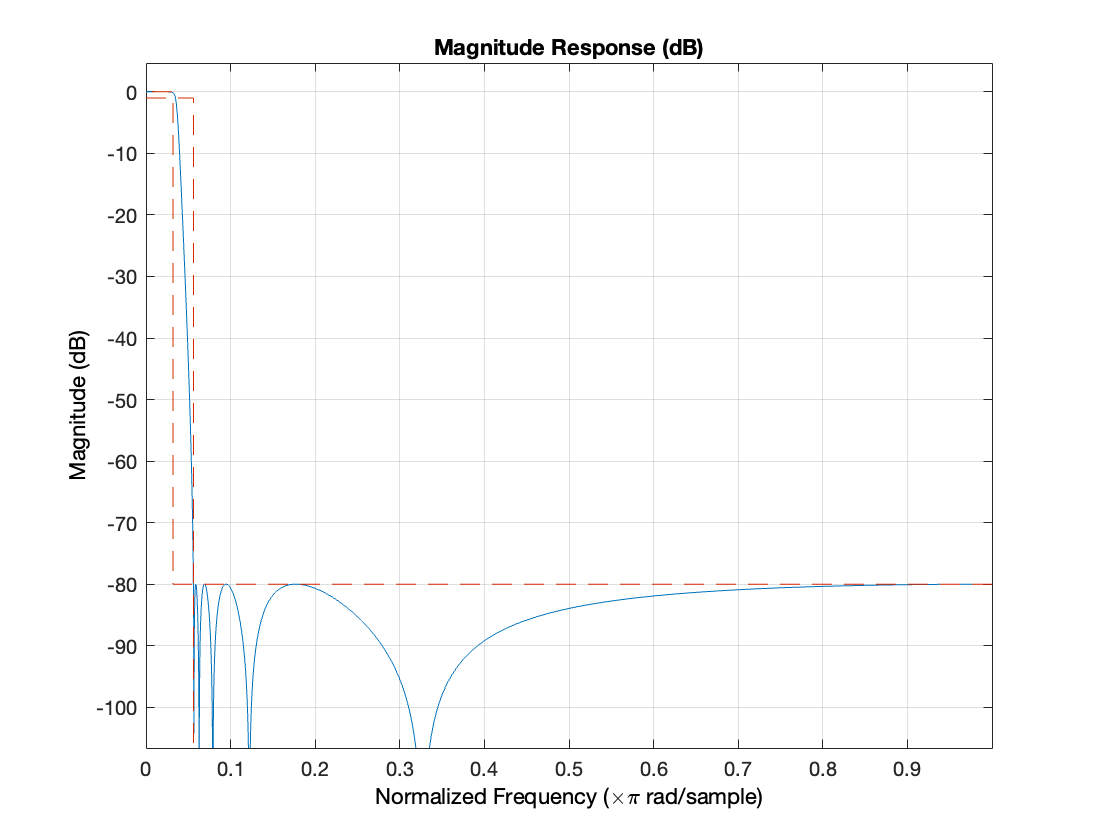
\includegraphics[width=\linewidth, trim={2.5cm, 1cm, 4cm, 1cm}, clip]{Figures/chebyII.png}
	\caption{Frequency response of IIR Chebyshev Type II.}
	\label{fig:cheby}
\end{figure}

\begin{figure}[H]
	\centering
	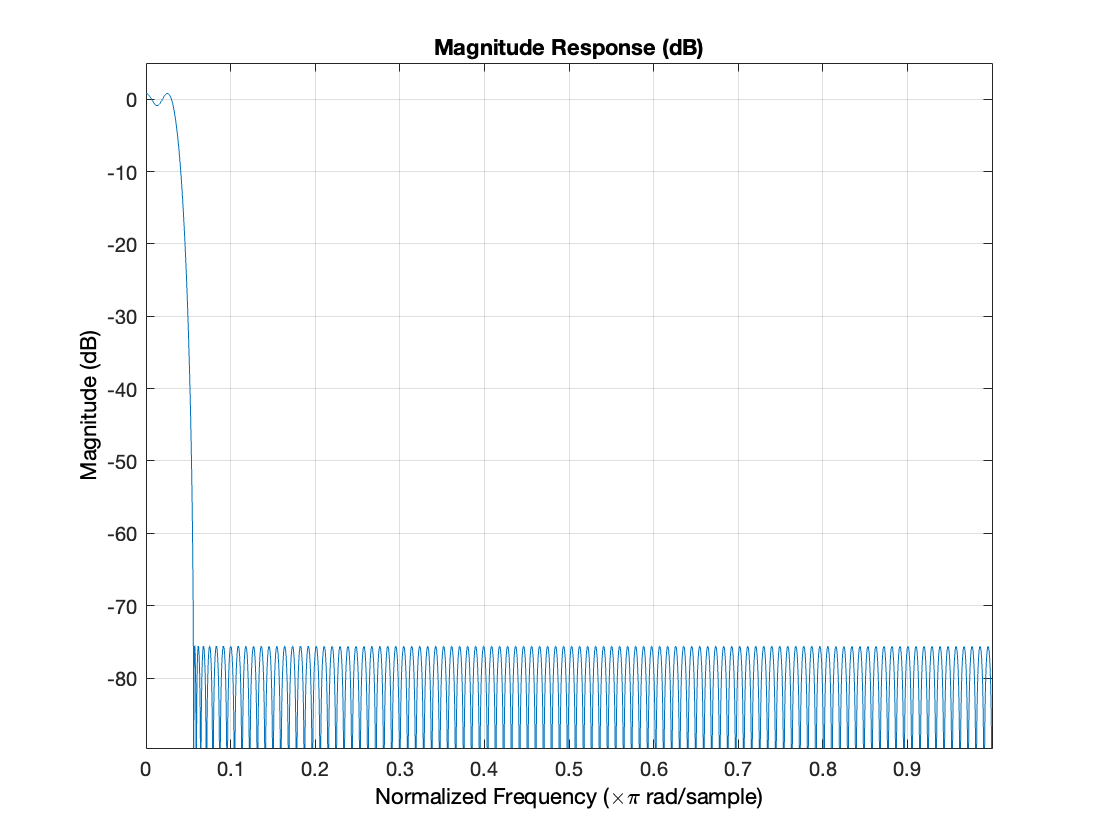
\includegraphics[width=\linewidth, trim={2.5cm, 1cm, 4cm, 1cm}, clip]{Figures/equiripple.png}
	\caption{Frequency response of FIR Equiripple.}
	\label{fig:equiripple}
\end{figure}


\subsection{Filter performance evaluation}
So that both filters could be compared objectively their power spectral denstity was computed. The discrete-time Fourier transform of a random signal's autocorrelation function $R_{xx}(k)$ is defined as its power spectrum $S_{xx}(\omega)$. The frequency content of the random signal $x(n)$ is represented by the power spectrum 
\begin{equation}
	S_{xx}(\omega) = \sum_{-\infty}^{\infty} R_{xx}(k)\cdot e^{-j\omega k},
\end{equation}
where $\omega = 2\pi f/f_s$ is the digital or normalized frequency in radians per sample.

Furthermore, the quantity $S_{xx}(f)/f_s$ represents the power per unit frequency interval, which describes the \emph{power spectrum} or \emph{power spectrum density}. It shows how the signal's power is spread out among the individual frequencies. \cite{orfanidis_introduction_1996}

The mentioned filters should have a large amount of their power in the pass-band region and much of the power in the stop-band region should be absent, so that the high frequency noise is attenuated. This observation is corroborated by an objective visual inspection of the power spectra of both filters. The power spectral density plots of both filters can be seen in Figure \ref{fig:powerspectra}.

\begin{figure}
	\centering
	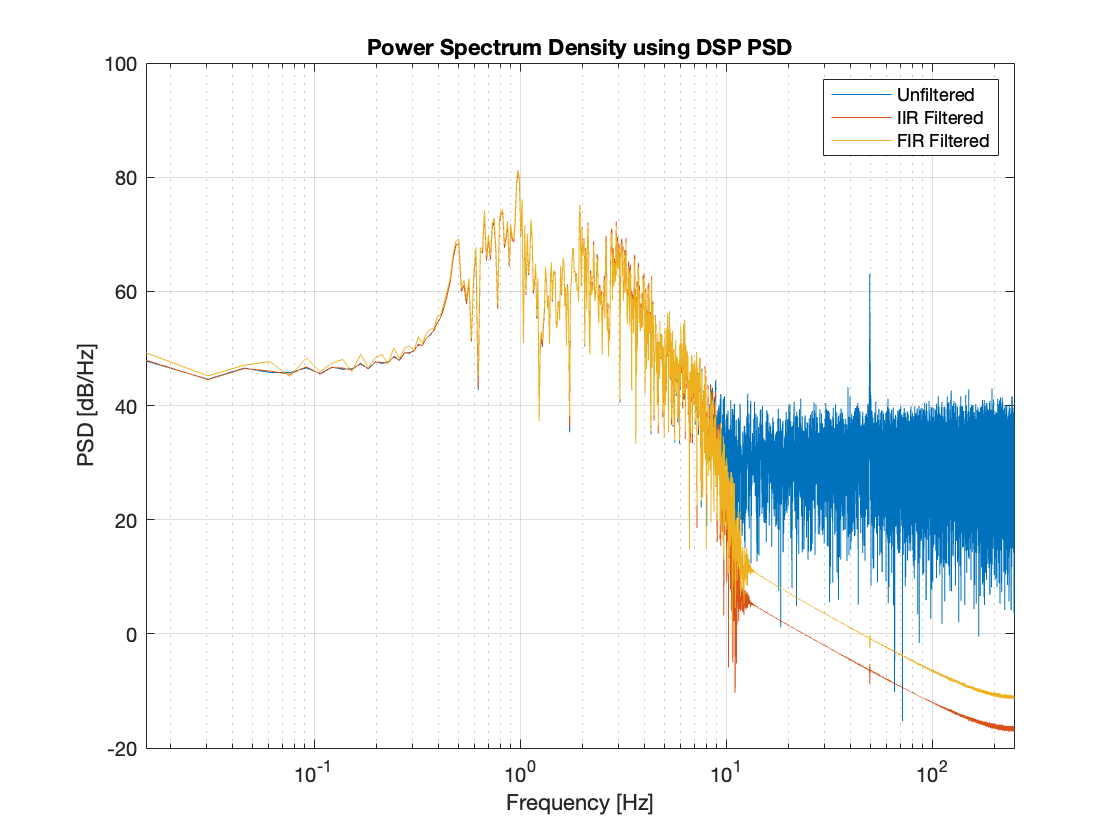
\includegraphics[width=\linewidth, trim={2.5cm, 1cm, 2cm, 1cm}, clip]{Figures/powerspectra.png}
	\caption{Power spectrum of the IIR Chebyshev Type II and FIR Equiripple filter compared to the unfiltered power spectrum.}
	\label{fig:powerspectra}
\end{figure}


\subsection{Heartbeat peak detection}
In order to detect peaks of the heartbeat signals, the derivative of the signal was needed and was computed via a simple algorithm based on a backward implicit finite difference method, as depicted in Equation \eqref{eq:finite_diff}
\begin{equation}\label{eq:finite_diff}
	u'(x) = \frac{u(x) - u(x-h)}{h},
\end{equation}
where $u(x)$ is the value of the current time sample, $u(x-h)$ is the value of the previous time sample two samples ago and $h$ is the distance between each time sample, which was $1/fs$. 

To classify a peak, the following criteria were employed: the signal had to reach a threshold value equaling 40\% of the maximum signal value, and the derivative of the signal needed to lie within $\pm5\%$ of the maximum and minimum derivative values. To prevent multiple detections within a short interval, a waiting period of 200 samples was enforced. If these conditions were met, the index was classified as a peak. Given the above conditions, if the PPG signal values were to decrease significantly, subsequent peaks might fail to be detected. To correct for this potential issue, the peak threshold was reset after a duration of $2f_s$, establishing a new threshold based on the current maximum value. The algorithm was evaluated through visual inspection of the marked peaks. An interval of 10 seconds can be seen in Figure \ref{fig:peaks}.
\begin{figure}
\centering
	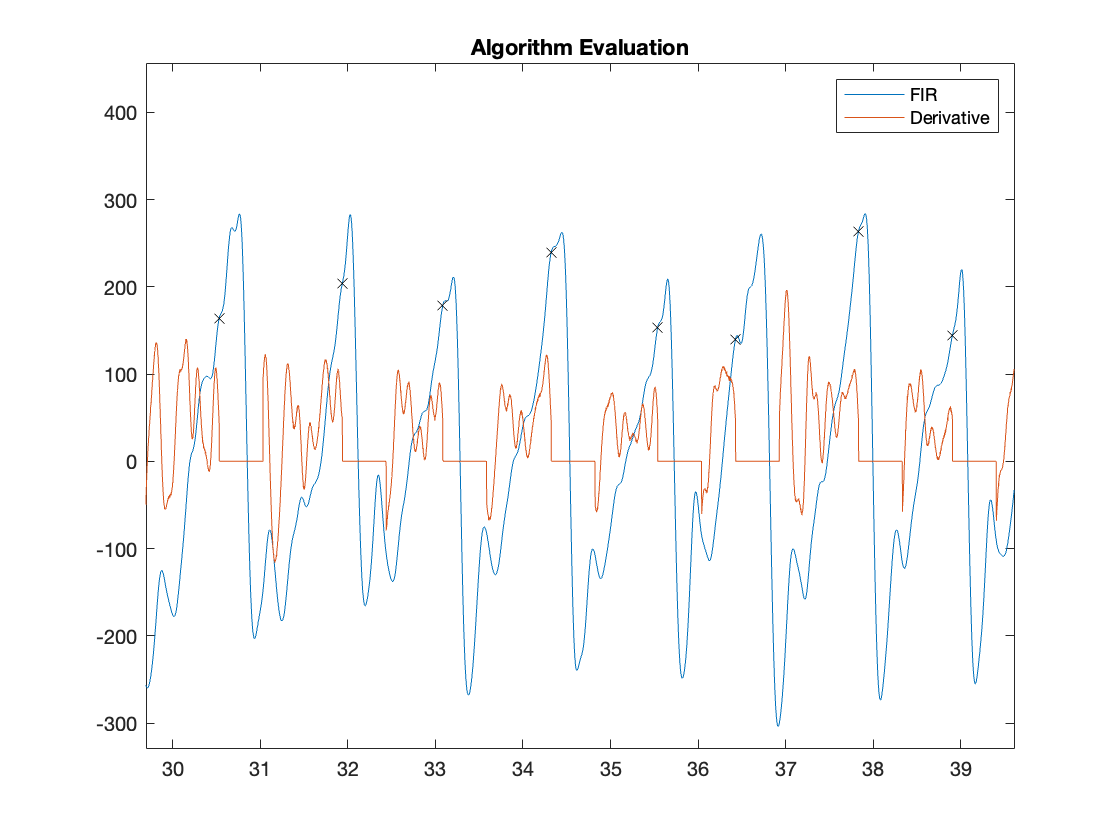
\includegraphics[width=\linewidth, trim={2.5cm, 1cm, 2cm, 1cm}, clip]{Figures/peaks.png}
	\caption{Evaluation of the heartbeat peak detection algorithm.}
	\label{fig:peaks}
\end{figure}
In order to evaluate the algorithm the peaks were counted manually and then compared to the number of peaks detected by it. The evaluation of the MATLAB implementation can be found in the results.

\subsection{Heart rate calculation}
The heart rate was computed during intervals of $15f_s$, where the number of peaks was divided by the number of intervals and then multiplied by $60$ in order to compute the heart rate in [beats per minute].

\subsection{Microcontroller porting}
After the peak detection algorithm was tested in MATLAB, the algorithm was programmed in C and ported onto the microcontroller. 

\subsection{Sensitivity of peak detection algorithm}
In order to get some sort of a metric to describe the performance of the implemented heartbeat peak detection algorithm, the sensitivity was calculated using Equation \eqref{eqn:accuracyEquation}

\begin{equation}
	\label{eqn:accuracyEquation}
	\text{Sensitivity} = \frac{TP}{TP+FN} \times 100 \%.
\end{equation}

where $TP$ is the number of true positives (i.e. the algorithm correctly identified a heartbeat peak) and $FN$ is the number of false negatives (i.e. the algorithm was unable to identify a heartbeat peak) \cite{trevethan_sensitivity_2017}.













\newcommand{\RNum}[1]{\uppercase\expandafter{\romannumeral #1\relax}}

\section{Results}

\setlength{\tabcolsep}{3pt}
\begin{table}[ht]
	\begin{flushleft}
		\caption{Comparison of segmentation performance between Random Forest and Atlas-based methods.}
		\begin{tabularx}{\linewidth}{Xcccc}
			\toprule
			\multirow{2}{*}{Region} & \multicolumn{2}{c}{Random Forest} & \multicolumn{2}{c}{Atlas} \\ 
			\cmidrule(lr){2-3} \cmidrule(lr){4-5}
			\midrule
			Noise & No & Yes & No & Yes \\
			Amygdala & $0.47 \pm 0.06$ & $0.47 \pm 0.06$ & $\mathbf{0.63 \pm 0.08}$ & $0.61 \pm 0.07$ \\
			Hippocampus & $0.43 \pm 0.05$ & $0.43 \pm 0.06$ & $0.61 \pm 0.10$ & $\mathbf{0.63 \pm 0.06}$ \\
			Thalamus & $0.68 \pm 0.10$ & $0.68 \pm 0.10$ & $\mathbf{0.79\pm 0.04}$ & $0.78 \pm 0.05$ \\
			Grey Matter & $0.73 \pm 0.01$ & $\mathbf{0.74 \pm 0.01}$ & $0.53 \pm 0.02 $ & $0.52 \pm 0.03$ \\
			White Matter & $\mathbf{0.83 \pm 0.02}$ & $\mathbf{0.83 \pm 0.02}$ & $0.66 \pm 0.03$ & $0.66 \pm 0.03$ \\
			Time (s)  & $197.3 \pm 6.3$  & $204.4 \pm 7.3$  & $6.0 \pm 1.8$  & $\mathbf{5.8 \pm 0.7}$ \\
			\bottomrule
		\end{tabularx}
	\end{flushleft}	
	\label{tab:performance_comparison}
\end{table}

The comparison of segmentation performance between the Random Forest-based and Atlas-based methods, both with and without noise, revealed distinct trends across brain regions. These differences can be seen in Table \RNum{1}. For the amygdala, the Atlas-based method without noise achieved the highest Dice score (0.63 ± 0.08) compared to the Random Forest method (0.47 ± 0.06). With noise, the Atlas-based method scored slightly lower (0.61 ± 0.07) but still outperformed the Random Forest method (0.47 ± 0.06). Similarly, for the hippocampus, the Atlas-based method performed better in noisy conditions, achieving the highest Dice score (0.63 ± 0.06) compared to the performance without noise (0.61 ± 0.10), while the Random Forest method showed no variability, scoring consistently (0.43 ± 0.05).
In the thalamus, the Atlas-based method achieved the best performance without noise (0.79 ± 0.04), slightly decreasing in the presence of noise (0.78 ± 0.05), whereas the Random Forest method showed consistent performance (0.68 ± 0.10) across conditions. Contrastingly, for grey matter, the Random Forest method performed better with noise (0.74 ± 0.01) than without noise (0.73 ± 0.01), while the Atlas-based method performed significantly worse, scoring 0.53 ± 0.02 without noise and 0.52 ± 0.03 with noise. For white matter, the Random Forest method outperformed the Atlas-based method with a consistent Dice score of 0.83 ± 0.02 across noise conditions, whereas the Atlas-based method achieved 0.66 ± 0.03 in both cases.
Regarding computational time, the Atlas-based method was significantly faster, taking 6.0 ± 1.8 seconds without noise and 5.8 ± 0.7 seconds with noise. In contrast, the Random Forest method required substantially more time, taking 197.3 ± 6.3 seconds without noise and 209.0 ± 7.5 seconds with noise. These results demonstrate clear differences in segmentation performance and computational efficiency between the two methods.

\section{Discussion}
The results presented in this study provide an insightful comparison between the Random Forest and Atlas-based methods for brain tissue segmentation. These findings reveal that each method has its strengths and weaknesses, which are highly dependent on the target brain structures and the computational resources available.

The Random Forest method demonstrated superior performance in segmenting larger structures, such as white matter and grey matter, primarily due to the type of features used in the classification process. Features capturing intensity, texture, and spatial distribution play a key role in distinguishing tissue types (CITATION NEEDED). Larger structures like white matter tend to exhibit more uniform and distinctive intensity patterns, which are more easily captured by statistical features such as mean intensity and variance. Additionally, textural features, which quantify patterns and variations, are more consistent and pronounced in larger regions, making them easier to classify. In contrast, smaller structures, such as the thalamus, present challenges due to their limited size and less distinct textural properties. The statistical sampling of features in Random Forest models is designed to handle diverse and high-dimensional data, but smaller structures contribute fewer representative samples during the training process. This imbalance can lead to a bias in favor of larger structures that dominate the feature set. Consequently, the Random Forest method's reliance on a multidimensional feature set enables it to excel in segmenting larger regions where spatial and intensity variations are more readily learned, while smaller regions remain more challenging to classify accurately.

The Atlas-based method showed better performance in segmenting smaller structures, such as the thalamus, which exhibit a high degree of consistency in shape, size, and position across subjects (CITATION NEEDED). This anatomical consistency makes these structures particularly well-suited for atlas-based approaches. The compact, ellipsoid shape of the thalamus further simplifies segmentation, reducing the likelihood of errors. Additionally, the method’s reduced sensitivity to minor global misalignments ensures that even if the overall brain alignment is slightly off, the localized region around the thalamus can still align well. When the atlas registration is performed accurately, these factors enable reliable identification of the thalamus and other similar structures (CITATION NEEDED). The inherent simplicity of the atlas-based method, which does not require a complex classifier, enhances its effectiveness for smaller, well-defined regions that are consistently identifiable across subjects. However Atlas-based method had difficulty segmenting grey matter, as evidenced by the lower Dice scores in this region, and also performed poorly with white matter compared to the Random Forest method. Grey matter presents a unique challenge because it is not as homogeneous as other tissue types (CITATION NEEDED), with complex anatomical boundaries and high variability between individuals in terms of size and shape (CITATION NEEDED). Similarly, white matter segmentation suffers from low contrast with neighboring tissues and partial volume effects, which blur boundaries and reduce segmentation accuracy.

Additionally, the atlas-based method's reliance on the quality of the initial atlas can limit its performance for both grey and white matter. If the atlas was constructed from a population with different anatomical characteristics than the study dataset, segmentation accuracy may degrade significantly. The widespread and convoluted nature of grey matter, along with the complex organization of white matter tracts, increases sensitivity to registration errors. Misalignments during registration can lead to compounded inaccuracies, particularly for larger, less consistent structures like white matter. Furthermore, the static nature of the atlas-based method prevents it from adapting dynamically to individual anatomical variability, unlike the Random Forest method, which leverages a large and diverse training dataset to flexibly address such variations and therefore produces more accurate segmentations for both grey and white matter.

In addition to segmentation performance, computational efficiency is a key consideration. The Atlas-based method was significantly faster, completing segmentation in seconds compared to the minutes required by the Random Forest method. This efficiency stems from its reliance on predefined atlases and transformations, involving only resampling and registration steps, making it ideal for large datasets. This speed advantage is critical in clinical settings, where rapid processing is often necessary (CITATION NEEDED). In contrast, the Random Forest method’s extensive training and prediction steps make it more computationally demanding and less suitable for real-time applications without further optimization.


Both methods demonstrated robustness against salt and pepper noise, maintaining segmentation performance despite image disruptions. While it is expected that the Atlas-based method, relying on spatial registration, would handle noise well if the process is robust, the Random Forest method's resilience was more surprising. Notably, the Random Forest performed well on salt and pepper test images even when trained solely on normal data, showcasing its ability to generalize effectively to noisy conditions. This highlights an unexpected strength, particularly valuable in real-world applications where medical images often contain noise from artifacts or patient movement (CITATION NEEDED).

The study has several limitations that must be considered. First, the dataset used in this study may not fully capture the variability in brain anatomy across different populations, such as those with diverse age groups or pathologies. This limitation could affect the generalizability of the findings to broader clinical settings. Second, the Atlas-based method’s performance heavily depends on accurate registration, and misalignments can significantly degrade segmentation quality, particularly in regions with high inter-subject variability. To address this, future work could involve constructing multiple atlases tailored to specific populations, allowing better capture of anatomical variations and improving segmentation accuracy. Lastly, while both methods were robust to salt and pepper noise, their resilience to other noise types, such as Gaussian or motion artifacts, was not evaluated, leaving their performance under such conditions uncertain.
\section{Conclusion}
\section*{Acknowledgment}

%We would like to express our appreciation for the teachings of Professor Mauricio Reyes who, through his engaging and though-provoking lectures for the Medical Image Analysis course, has given us a solid understand of the current knowledge in the field. We would also like to extend our heartfelt thanks to Shelley Shu and Amith Kamath for their guidance throughout this project and for creating a very enjoyable learning environment during the lab.

We would like to extend our heartfelt thanks to Shelley Shu and Amith Kamath for their guidance throughout this project and for fostering an engaging and enjoyable learning atmosphere during the lab. We would also like to express our sincere thanks to Professor Mauricio Reyes for imparting us with valuable knowledge throughout the lectures of the Medical Image Analysis course.

%----------------------------------------------------------------------------------------
%	 REFERENCES
%----------------------------------------------------------------------------------------

\printbibliography % Output the bibliography

%----------------------------------------------------------------------------------------

\end{document}
